%!TEX TS-program = xelatex
\documentclass[]{friggeri-cv}
\usepackage{afterpage}
\usepackage{hyperref}
\usepackage{color}
\usepackage{xcolor}
\usepackage{fontspec}
\usepackage[utf8]{inputenc}

\hypersetup{
    pdftitle={Wesley Banfield CV},
    pdfauthor={Wesley Banfield},
    pdfsubject={CV},
    pdfkeywords={CV Wesley Banfield},
    colorlinks=false,           % no lik border color
    allbordercolors=white       % white border color for all
}

\RequirePackage{xcolor}
\definecolor{pblue}{HTML}{0395DE}

\begin{document}

\begin{figure}[!h]
	\begin{minipage}{0.48\textwidth}
		\begin{flushleft}
			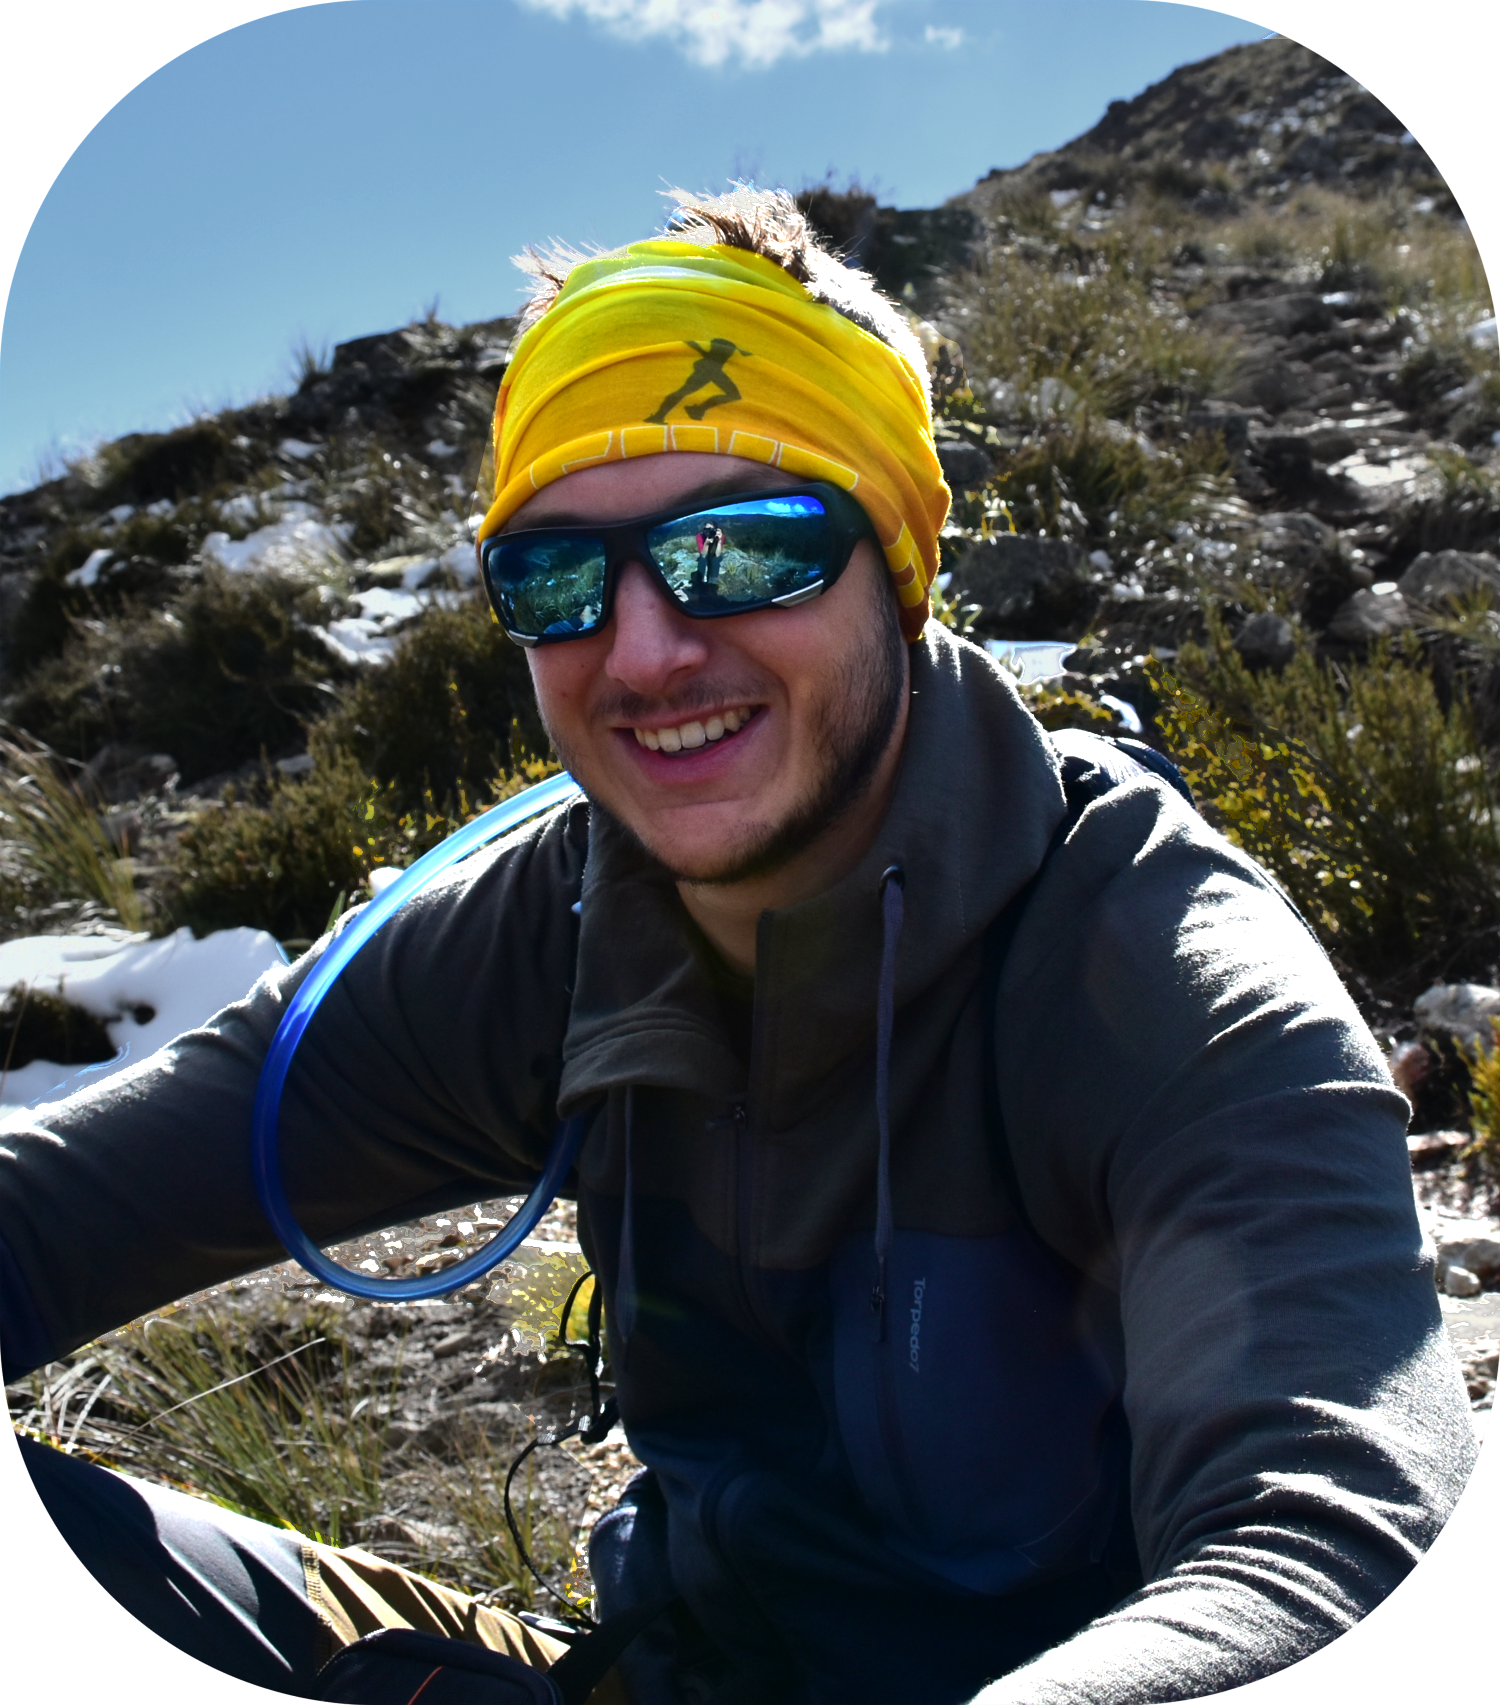
\includegraphics[width=2.75cm]{img/profile_relaxed.png}
		\end{flushleft}
	\end{minipage}\hfill
	\header{Wesley}{ Banfield}
 	{Unconventional Thinker - Geologist - Software Engineer}
	\begin{minipage}{0.48\textwidth}
		\begin{flushright}
			
\includegraphics[width=2.75cm]{img/QR.png}
		\end{flushright}
	\end{minipage}
\end{figure}
\vspace{-0.75cm}
% Fake text to add separator      
\fcolorbox{white}{gray}{\parbox{\dimexpr\textwidth-2\fboxsep-2\fboxrule}{%
.....
}}

\begin{quote}
\large
\begin{center}
Innovative engineer looking to \textbf{unite cutting edge web technologies and geosciences} to help provide a more sustainable future.
\\
\end{center}
\end{quote}

\begin{center}
\vspace{6pt}
\href{mailto:wesleybanfield@gmail.com}{\textbf{wesleybanfield@gmail.com}}
\\+33 7 83 87 38 09, Lyon, France
\\\emph{GB / USA citizen, FR bilingual}
\vspace{3pt}
\\\href{https://www.linkedin.com/in/wesleybanfield/}{LinkedIn},
\href{https://github.com/WesleyTheGeolien}{GitHub}
\end{center}

\vspace{6pt}
\begin{table}[!h]
	\centering
	\begin{tabular}{L{3.25cm}cL{2cm}L{2.25cm}cL{2cm}L{2.25cm}c}
		\multicolumn{2}{c}{\large\textbf{\textcolor{pblue}{Technologies}}} && \multicolumn{2}{c}{\large\textbf{\textcolor{pblue}{Languages}}} && \multicolumn{2}{c}{\large\textbf{\textcolor{pblue}{Software Development}}} \\
		\textbf{Containerization / Micro-services} & 
\includegraphics[scale=0.40]{img/5stars.png} && \textbf{Python} & 
\includegraphics[scale=0.40]{img/5stars.png} && \textbf{Full Stack} & 
\includegraphics[scale=0.40]{img/4stars.png} \\
		\textbf{Interactive Web Tools} &  
\includegraphics[scale=0.40]{img/4stars.png} &&
		\textbf{Javascript / HTML} & 
\includegraphics[scale=0.4]{img/4stars.png} &&
		\textbf{APIs / Database Calls} & 
\includegraphics[scale=0.40]{img/4stars.png} \\
		\textbf{Flask} & 
\includegraphics[scale=0.40]{img/4stars.png} &&
		\textbf{C++ / Fortran} & 
\includegraphics[scale=0.4]{img/3stars.png} &&
		\textbf{Backend Compute} & 
\includegraphics[scale=0.40]{img/4stars.png} \\
		\textbf{Jupyter} & 
\includegraphics[scale=0.40]{img/4stars.png} && 
		\textbf{SQL} & 
\includegraphics[scale=0.4]{img/4stars.png}
		&&
		\textbf{Frontend} & 
\includegraphics[scale=0.40]{img/4stars.png} \\
		\textbf{Parallelization / Sharding} &
		
\includegraphics[scale=0.40]{img/3stars.png} &&
		\textbf{\LaTeX} & 
\includegraphics[scale=0.4]{img/4stars.png}
		&&
		\textbf{Database Design}&
		
\includegraphics[scale=0.40]{img/3stars.png}\\
	\end{tabular}
\end{table}
\vspace*{\fill}
\section{Experience}
\begin{entrylist}
  \entry
  {9/20 - Now}
  {Research Engineer - Climate}
  {\href{https://cerege-cl.github.io/}{Protisvalor - CEREGE}}
  {Climate Simulations pose multiple technical problems from the setting up boundary of conditions to the interpretation of results.
  \\[3pt]
  As part of the paleo-climate team I lead the development of an \href{https://cerege-cl.github.io/netcdf_editor_app/}{open source interactive web based tool} to setup boundary conditions for the IPSL model. Relying on a micro-service architecture and messaging queues, complex compute is carried in multiple languages in different containers. The tool is used by the greater climate community for the ability to interactively edit NetCDF files.
  \\[3pt]
  Often simulation results are too large to manage on a local machine. I deployed and maintain the JupyterHub server for the group providing team members with a unified functional development environment and sufficient compute resources.
  \\[3pt]
  In a research environment outreach is crucial, to that end I designed and deployed the \href{https://cerege-cl.github.io/}{teams web portal.}}
  \entry
  {10/19 - 6/20}
  {Project Manager Digital Innovation}
  {\href{http://envisol.net/}{Envisol, France}}
  {In charge of designing and developing the front and backend of internal and market-ready web-based tools for data acquisition and interpretation for the Contamination and Remediation industry. Automation GIS data collection and treatment through web services.}
  \entry
    {01/17 - 05/19}
    {Research Engineer}
    {\href{https://www.seequent.com/}{Seequent, Christchurch New Zealand}}
    {I pride myself on thinking laterally and outside of the box to provide novel innovative solutions, drawing on insights from both my geological and software engineering backgrounds.
    \\[3pt]
    The role permitted vast exposure to the company and clients. Regular client meetings and presentations were held as well as working, and leading, interdisciplinary initiatives.
    \\[3pt]
    Seequent are the developers of the \href{https://www.leapfrog3d.com/}{Leapfrog Suite}, a world standard for 3D implicit geological modelling software. Daily use and technical insights led me to become an expert user, continuously pushing the limits.
    \\[6pt]
}
        \end{entrylist}
    \vspace*{\fill}
    \newpage
    \vspace*{18pt}
\begin{entrylist}
	\entry{}{}{}{
   	\textbf{New Technologies} Some problems call for thinking outside the box and implementing new technologies from the base up. Examples of these projects included web based dashboard creation, integration of Jupyter into workflows and deploying compute intensive tasks to the cloud.
   	\\[6pt]
   	\textbf{New Solutions} Other projects included the reuse of core IP in novel manners. For example the automated creation of geological models from sub sets of data to sample geological uncertainty. This work was presented at Seequent's \href{https://www.youtube.com/watch?v=jt26J5ljlA0}{Perth Lyceum}.
    \\[6pt]
   	\textbf{Core Strategy} Providing technical support for key business decisions including full verification of geostatistical implementations and creation of infrastructure to obtain and analyse usage metrics of Leapfrog software. 
    \\
    Reference : \href{mailto:tim.schurr@seequent.com}{Tim Schurr, Solutions Architect}
	}
  \entry
    {05/16 - 09/16}
    {Software Integration Engineering Internship}
    {\href{https://www.total.com/en}{Total, Pau France}}
    {Discretization plays an important part in coupled Oil \& Gas basin modelling. Too fine, the computation time prevails, too coarse and the calculations do not converge. As a software integration engineer I implemented an interface with the \href{http://www.ring-team.org/software/ringmesh}{RINGMesh} library to dynamically re-mesh during simulations.\\ Reference : \href{mailto:tristan.cornu@total.com}{Tristan Cornu, Pore pressure and Rock Mechanics Specialist}}

    \entry
    {02/16 - 05/16}
    {Research Intern}
    {\href{http://www.ring-team.org/}{Ring Research Lab, Nancy France }}
    {Research and implementation of different automatic simultaneous well log correlation algorithms and creation of a SKUA-Gocad plug-in. The master's thesis was carried out in the lab that originally developed SKUA-Gocad before commercialisation by Paradigm. The work was presented and published in the 2016 Ring Meeting. \\Reference : \href{mailto:Guillaume.Caumon@ensg.univ-lorraine.fr}{Dr. Guillaume Caumon, Head of Research team}}
    \entry
    {06/15 - 09/15}
    {Software Engineering Internship}
    {\href{https://www.seequent.com/}{Seequent, Christchurch New Zealand}}
    {Design and development of a graphical user interface for geostatistical analysis in Leapfrog 3D Geological modelling suite, later integrated into Leapfrog EDGE. Implementation of different geostatistical algorithms.
    \\
    Reference : \href{mailto:tim.mclennan@seequent.com}{Tim McLennan}}

	\entry
	{09/14 - 05/15}
	{Lab Research Project}
	{\href{http://georessources.univ-lorraine.fr/}{GeoRessources, Nancy France}}
	{Geochemistry can be used to date oil, however when in contact with water certain couples reset. The goal of the project was to develop an experimental protocol to analyse the behaviour of the Rhenium / Osmium couple. Automated graphing tools where developed to analyse the ICP-MS results.
		\\
		Reference : Raymond Michels}
\end{entrylist}
\section{Presentations and Publications}
\begin{entrylist}
	\entry
	{2021}
	{Portable interactive Plotting with Javascript}
	{Software Underground}
	{1h30 talk on how to use Python with Javascript to create portable graphs that can be used in any web browser. Viewable on \href{https://www.youtube.com/watch?v=j\_4wkMzGvKs}{YouTube}}
	\entry
	{2020}
	{Prototyping for Geologists}
	{Transform 2020}
	{Short talk on building a infrastructure to rapidily build and deploy prototypes.
	Viewable on \href{https://youtu.be/rUbvueIF5f8?t=4130}{YouTube}.}
	\entry
	{2019}
	{JupyterLab Quick Start Guide}
	{Packt}
	{Coauthor of the book written for Packt aimed at familairzing data scientists with the next-generation web-based data science notebook and natural evolution of Jupyter. }
	\entry
	{2019}
	{Integration of BIM and the subsurface}
	{Indura Cluster}
	{Oral Presentation on behave of Envisol demonstrating the integrations between Building Information Modelling and subsurface data}
	\entry
	{2018}
	{How certain are you of your surfaces}
	{Seequent Lyceum Perth}
	{Oral Presentation in front of over 200 mining experts on behalf of Seequent demonstarting the latest R\&D work carried out at the company. Viewable on \href{https://www.youtube.com/watch?v=jt26J5ljlA0}{YouTube}.}
	\entry
	{2016}
	{Current automatic well log correlation techniques}
	{Ring Consortium}
	{Oral Presentation in front off over 100 Oil and Gas experts demonstarting my Master's thesis on automated well log correlation techniques. The Master's thesis was also published in the Proceedings.}
\end{entrylist}
\vspace*{\fill}
\newpage
\vspace*{18pt}
\section{Open Source Contributions}
\begin{entrylist}
	\entry
	{2021}
	{Seismic Footprint removal Hackathon}
	{Transform 2021}
	{Build a tool to design filters for seismic data in the frequency domain. After the hackathon a web based tool (panel) was built and deployed to AWS.}
	\entry
	{2020 - Now}
	{Pangeo collaborator}
	{Pangeo}
	{Take part in weekly catchups to discuss and better understand the intersection between computing and climate sciences}
	\entry
	{2020 - Now}
	{SOS Mediterranée website update}
	{CartONG}
	{Refresh of the website to show boat rescues in the mediterranean sea.}
	\entry
	{2020}
	{Well Correlation tool}
	{Transform 2020}
	{Build a web tool (Dash / plotly) to load LAS files and visualise them.}
\end{entrylist}
\section{Education MEng, MSc}
\begin{entrylist}
  \entry
    {2013 - 2016}
    {Master in Geological Engineering with specialisation}
    {\href{http://ensg.univ-lorraine.fr/english/}{French National School of Geological Engineering}}
    {\emph{Ecole Nationale Superieure de Geologie} is a leading French engineering school specialising in geosciences and delivering an Engineering diploma combined with a Master from the University of Lorraine.\\ 
    \\
    \emph{Curriculum}: Numerical Geology\\ 
    \emph{Natural Sciences}: Hyrdogeology, Structural Geology, Geomorphology, Geophysics\\
    \emph{Engineering Sciences}: Applied Maths, Fluid Dynamics, Statistics, Partial Differential Equations\\
    \emph{Software Sciences}:  Software Development, Interface Design, Computer Geometry, Visualisation and Parallelism, Mathematical concepts of geomodelling, Finite Elementss\\
    \\
    \emph{Title of Thesis}: ”Current automatic well log correlation techniques, their advantages and drawbacks”.
    \emph{References}: Dr. Guillaume Caumon, Jonathan Edwards\\}
  \entry
    {2011 - 2013}
    {\href{https://en.wikipedia.org/wiki/Classe_preparatoire_aux_grandes_ecoles}{Classes Preparatoires aux Grandes Ecoles}}
    {Lycee Pierre de Fermat, Toulouse France}
    {2 years of intensive general scientific courses before national exams for entry to the French Grandes Ecoles, carried out at Pierre de Fermat, one of the top preparatory schools finishing in the top 10\% nationally.\\ 
    \emph{Main subjects}: Mathematics, Physics, Chemistry, Biology and Geology, \\}
\end{entrylist}
\vspace*{\fill}
\end{document}